\documentclass[a4,12pt]{scrartcl}

%Basic 
\usepackage[utf8]{inputenc}
\usepackage[ngerman]{babel}
\usepackage[T1]{fontenc}
\usepackage{float}
\usepackage[bottom = 3.50cm]{geometry}

%Titel Seite
\title{CLOUD INFRASTRUCTURE}
\subtitle{Lab-07}
\author{Giorgio Vincenti \and Samuel Krieg}
\date{\today}


%Kopf, Fusszeile
\usepackage{fancyhdr}
\pagestyle{fancy}
\lhead{ \begin{picture}(0,0) \put(0,0){
\includegraphics[width=3cm]{./pictures/hsrlogo.png}} \end{picture}}
\chead{}
\rhead{Seite \thepage}
\lfoot{Cloud Infrastructure \\Lab-07}
\cfoot{Giorgio Vincenti \and Samuel Krieg}
\rfoot{\today}
\renewcommand{\headrulewidth}{0.4pt}

%Bilder
\usepackage{graphicx}

%Tabellen
\usepackage{booktabs}

%Codesnippets
\usepackage{listings}
\lstset{language=bash} 

%Querformat für eine Seite
\usepackage{lscape}
\usepackage{rotating}
\usepackage{pdflscape}

%Temp
\usepackage{lipsum}



\begin{document}

\clearpage\maketitle
\thispagestyle{empty}
\tableofcontents
\newpage

\section{Anforderungen an ein modernes Datacenter}
\subsection{Herausforderungen}
Die Herausforderungen in einem moderem Datacenter bestehen darin die riesigen Datenmengen, die generiert werden, effizient und schnell verarbeiten zu können. Die Storages und Server Performance spielen dabei eine grosse rolle, jedoch bringt diese Performance nichts, wenn das Netzwerk nicht dementsprechend mit den Datenmengen effizient umgehen kann. Die grossen Datenmengen verlassen das Datacenter nicht, sondern fliessen von System zu System.

\subsubsection{Beispiele}
Hier einige Beispiele in der Praxis. \\

\noindent \textbf{VMotion:} Zum Beispiel bei Einsatz von Virtualisierung muss der Administrator in der Lage sein, VMs über das Netzwerk auf andere Hosts innerst kürzester Zeit verschieben können. \\

\noindent \textbf{Webserver:} Ein anderes Beispiel bezieht sich auf ein Webserver/Datenbank Modell. Der Webserver muss Daten der Datenbank abfragen und abholen ohne grossen Verzögerungen.\\

\noindent \textbf{Backup:} Ein weiteres Beispiel betrifft die Backups der Maschinen. Da fliessen ebenfalls grosse Datenmengen übers Netzwerk. Falls mehrere Server innerhalb eines gewissen Zeitraums gesichert werden müssen, muss die Netzwerkperformance stimmen, damit keine Engpässe auftreten. 

\subsection{Anforderungen}
Die Anforderungen an ein solches Datacenter sind sehr hoch. Da gibt es einiges zu beachten: 
\begin{itemize}
\item Sehr hohe Verfügbarkeit 
\item Mobilität von Applikationen, Systemen und Daten
\item Zugriffe auf Applikationen, Systemen und Daten 
\item Hohe Auto-Skalierbarkeit 
\item Genaue Abrechnungen auf benutzte Dienste 
\item Sicherheit 
\item Hohe Performance 
\item Abhängigkeit 
\item Autoprovisioning von Applikationen, Systemen und Daten
\end{itemize}

\subsection{Netzwerkarchitektur}
Die Netzwerkarchitektur spielt eine sehr grosse Rolle in einem Datacenter. Auch diese bringt grosse Anforderungen mitsich, damit das Beste aus der Infrastruktur rausgeholt werden kann. 
\begin{itemize}
\item Skalierbarkeit
\item Performance 
\item Hohen Datendurchsatz zwischen den Systemen
\item Elephant-flows fähig 
\item Managebar 
\end{itemize}

\section{TRILL}
Trill steht für \textbf{Tr}ansparent \textbf{I}nterconnection of \textbf{L}ots of \textbf{L}inks und ist ein von der IETF festgelegten Standard.

\subsection{Funktion}
TRILL ist eine Kombination von Layer 2 (bridging) und Layer 3 (routing). Dank dieser Kombination ermöglicht TRILL ein routing auf Layer 2 zu betreiben. Wird ein Layer 2 Netzwerk auf Layer 3 betrieben, ist kein Spanning-Tree mehr notwendig.

\subsubsection{Implementation}
TRILL wird von  Geräte implementiert die sich RBridges (routing bridges) nennen. Ein anderer Name für diese Geräte ist TRILL Switches. 

\subsubsection{Routing}
Zwischen den verschiedenen RBridges wird ein Link State Routing Protokol eingesetzt, damit alle RBridges über die gesamte Netztopologie bescheid wissen. Dies ermöglicht den RBridges den optimalen Pfad zur Destination ausfindigzumachen. Als Protokoll wird IS-IS eingesetzt, weil es auf Layer 2 kommuniziert und somit keinerlei IP-Konfiguration benötigt und sehr leicht erweiterbar ist. TRILL erstellt eine separata IS-IS Instanz und ist von einer eventuell bestehenden Layer 3 IS-IS Instanz komplett losgelöst. Jede RBridge hat eine eindeutige IS-IS ID von 48 Bit, welche von der eigenen MAC-Adresse abgeleitet wird. 

\subsubsection{RBrigdes ID}
Jede RBrigde im Netzwerk hat eine eindeutige ID (Bridge Identifier). Diese ID wird entweder dynamisch gewählt, oder kann durch den Netzwerkadministrator statisch vergeben werden. 

\subsubsection{Loop Prevention}
Im TRILL Header existiert ein Feld das sich Hop Count nennt. Durch dieses Feld werden Loops verhindert. Die RBridges stellen das Hop Count Feld auf die erwartete anzahl Hops, und jede RBridge dekrementiert das Feld um 1. Bei 0 wird das Packet verworfen.  

\subsubsection{Encapsulation}
Die RBridge welches ein Ethernet Frame von einem Client erhält (ingress bridge) verpackt das Frame in ein TRILL Packet. Dabei wird der TRILL Header eingefügt (siehe nächstes Kapitel). In diesem Header wird die destination bridge (engress bridge) spezifiziert, welche das ankommende Packet wieder auspackt und es an den Client weiter sendet, welcher das Packet erhalten soll. Wie ein eingepacktes Frame aussieht, wird im nächsten Kapitel gezeigt. 

\subsubsection{VLAN-Tags}
VLAN kann trotz TRILL verwendet werden. Es wird zwischen zwei VLANs unterschieden. Im Inner Ethernet Header: Inner VLAN-Tag, im Outer Ethernet Header: Outer VLAN-Tag. Die VLAN-Tags werden von TRILL nicht verrändert. Das Inner VLAN-Tag ist das ursprüngliche VLAN des Clients. Der Outer VLAN-Tag wird von der RBridge gesetzt beim Versand des Packets. 

\subsection{Header}
Der Header von TRILL sieht gemäss RFC 6325 folgendermassen aus: 

\begin{figure} [H]
	\begin{center}
	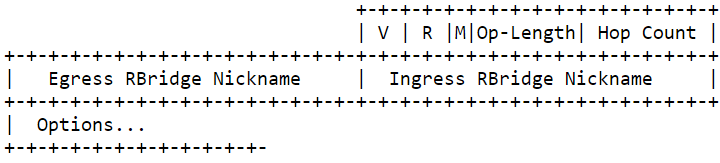
\includegraphics[width=0.80\textwidth]{./pictures/trill_header.png}
	\caption{TRILL Header aus RFC 6325}
	\label{x}
	\end{center}
\end{figure}

\subsubsection{Felder}
\begin{itemize}
\item V (Version: aktuell 0): 2 Bit
\item R (Reserved): 2 Bit.
\item M (Multi-destination: 1. Bit 0 = unicast, 2. Bit 1 = distribution tree): 2 Bit.
\item Op-Length (Options Length): 5 Bit
\item Hop Count(jede RBridge dekrementiert, bei 0 wird Paket verworfen): 6 Bit
\item Egress RBridge Nickname (source bridge): 16 Bit identifier
\item Ingress RBridge Nickname (destination bridge): 16 Bit identifier
\end{itemize}

\subsubsection{Encapsulation TRILL Frame}
Ein eingepacktes TRILL Frame sieht folgendermassen aus: (wurde aus RFC 6325 entnommen) 

\begin{figure} [H]
	\begin{center}
	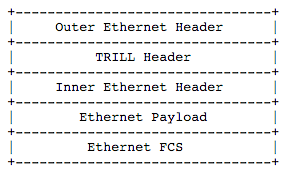
\includegraphics[width=0.80\textwidth]{./pictures/trill_encapsulation.png}
	\caption{An Ethernet Encapsulated TRILL Frame}
	\label{x}
	\end{center}
\end{figure}

\noindent Der Client sendet das Packet, welches aus Inner Ethernet Frame, Ethernet Payload und Ethernet FCS besteht, an die ingress bridge. Diese packt den TRILL Header obendrauf, welcher die engress brigde (destination bridge) enthält und sendet das Packet an die nächste RBridge. Bei jedem Hop wird der Outer Ethernet Header angepasst, je nach Source und Destination Adresse. Das restliche Packet bleibt erhalten, bis es bei der engress bridge ankommt. Da wird es entpackt und an den Client weitergesendet. 
\newpage

\noindent Hier eine detailliertere Abbildung eines Frames, das zwischen zwei RBridges ausgetauscht wird: (über zwei weitere RBridges) 
\begin{figure} [H]
	\begin{center}
	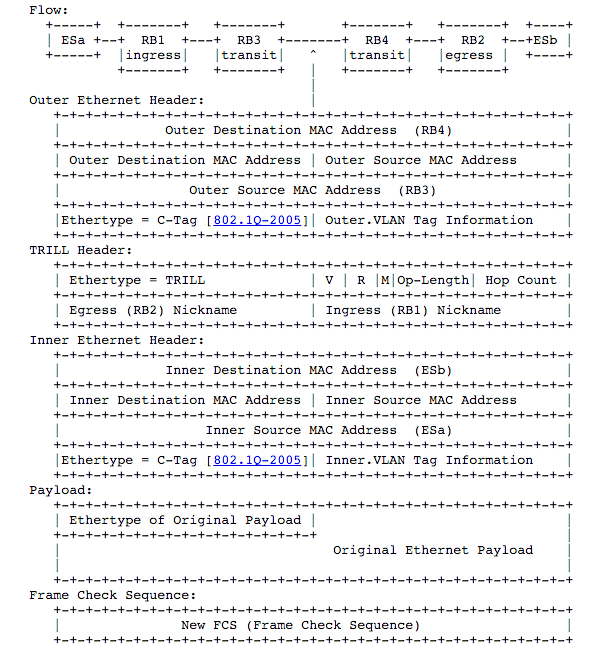
\includegraphics[width=0.80\textwidth]{./pictures/trill_frame_flow.png}
	\caption{TRILL Data Encapsulation over Ethernet}
	\label{x}
	\end{center}
\end{figure}

\noindent Anhand von dieser Grafik ist zu erkennen, das der Outer Ethernet Header nach jedem Hop geändert wird. In diesem Beispiel befindet sich das Packet zwischen RB3 und RB4. Dies bedeutet das im Outer Ethernet Header unter Destination RB4 steht, und unter Source RB3. Das restliche Packet ist unverrändert (abgesehen der Hop Count im TRILL Header, da wird dekrementiert nach jedem Hop). 
\newpage

\subsection{Ziele von TRILL}
Das Hauptziel von TRILL ist es ein Layer 2 Routing zu betreiben. Dadurch wird das Spanning-Tree Protokoll nicht weiter benötigt, das in Rechenzentren inakzeptable Aussetzer verursachen würde. TRILL kann einfach auch in bestehende Netzwerke eingesetzt werden, in dem nicht alle Geräte TRILL unterstützen. 

\subsection{Wieso wurde TRILL entwickelt?}
TRILL wurde entwickelt um Spanning-Tree in kritische Umgebungen ablösen zu können. Spanning-Tree ist nicht gut geeignet da es die ungenutzte Pfade blockiert um loops zu vermeiden. Dadurch kann nicht die volle Bandbreite genutzt werden und im Falle eines Ausfalls, benötigt Spanning-Tree einige Zeit um den blockierten Pfad aufzuheben. Dadurch können Unterbrüche und Verzögerungen entstehen, welche in einem Rechenzentrum nicht erwünscht sind. TRILL behebt dieses Problem. Bei TRILL gibt es keine blockierten Pfade, somit kann die gesamte Bandbreite genutzt werden. TRILL betreibt im Gegensatz zu STP ein Layer 2 Routing, was dazuführt das keine Loops entstehen können. Das STP und das TRILL wurden beide von der gleichen Entwicklerin designed, und zwar von Radia Perlmann. 

\subsection{Wo kann TRILL eingesetzt werden?}
Der Einsatz von TRILL macht bei diverse Szenarien Sinn: 
\begin{itemize}
\item In Rechenzentren wo hohe Bandbreiten und Verfügbarkeit gefragt sind (da TRILL keine Pfade blockt, und keine Unterbrüche verursacht bei aktivieren der blockierten Pfade wie STP) 
\item In Rechenzentren wo virtuelle Maschinen flexibel verschiebt werden müssen
\item In Netzwerke wo nicht alle Geräte TRILL unterstützen (die Geräte die kein TRILL unterstützen, sehen die TRILL RBridges als einzigen Switch und reden STP mit diesem)
\item In allen Netzwerke wo STP im Allgemeinen nicht erwünscht ist 
\item In Netzwerke in welchem ein verlängertes Layer 2 Netzwerk benötigt wird 
\item In allen Netzwerken in welchem Layer 2 Routing notwendig ist 
\end{itemize}

\subsection{Vergleich von TRILL mit traditionelle Protokolle}
\subsubsection{Spanning-Tree}
TRILL ist sicher mit Spanning-Tree vergleichbar, da TRILL dazu entwickelt wurde Spanning-Tree abzulösen. \newpage
\textbf{Limitationen}
\begin{itemize}
\item Da TRILL das STP Protokoll ablösen soll, gibt es keine Limitationen. Ein einziger Punkt ist sicher das STP viel weiter verbreitet und viel mehr unterstützt wird. 
\end{itemize}
\textbf{Unterschiede}
\begin{itemize}
\item TRILL hat im Gegensatz zu STP ein Hop Count Feld. 
\item Die Packete werden von den RBridges eingepackt mit einem TRILL Header
\item TRILL blockiert keine Pfade um Loops zu vermeiden 
\item TRILL funktioniert als Layer 2 Routing 
\item TRILL noch nicht soweit verbreitet wie STP 
\end{itemize}

\subsubsection{Shortest Path Bridging (SPB)}
Ein sehr ähnliches Protokoll ist SPB.  \\
\textbf{Limitationen}
\begin{itemize}
\item SPB Modus für normale VLAN Bridges, TRILL redet da von TRILL Domain
\item TRILL performanter als SPB 
\end{itemize}
\textbf{Unterschiede}
\begin{itemize}
\item TRILL wurde von IETF veröffentlich, SPB von IEEE
\item SPB Nachfolgder von PBB (gibt es schon länger) 
\end{itemize}

\subsection{Welche Vor- und Nachteile bringt TRILL mit sich?}
Wie jedes Protokoll gibt es Vor- und Nachteile. 
\subsubsection{Vorteile}
\begin{itemize}
\item Spanning-Tree nicht mehr notwendig 
\item keine blockierte Verbindung mehr (kein STP) 
\item keine Unterbrüche bei Link Ausfall (kein STP)
\item Alle Links können aktiv genutzt werden (kein STP) 
\item Sehr gut Skalierbar 
\item Nicht alle Geräte müssen TRILL unterstützen um es betreiben zu können
\item Kein fundiertes Wissen über IS-IS notwendig   
\item Layer 2 Routing 
\end{itemize}
\subsubsection{Nachteile}
\begin{itemize}
\item Noch nicht weit verbreitet 
\item Nicht von allen Geräte unterstützt 
\item Oft wird nicht TRILL integriert sondern Hersteller ähnliche Protokolle 
\end{itemize}

\subsection{Ähnliche Technologien wie TRILL} 
Eine Alternative zu TRILL ist das Shortest Path Protocol (SPB), dass von IEEE entwickelt wurde. Beide Protokolle wurden dazu entwickelt STP in Rechenzentren zu ersetzten, und beide verwenden IS-IS. SBP unterstützt ebenfalls Multipath-Routing, und ist optimal für grosse Layer 2 Netzwerke mit vielen Verbindungen. Hier eine Vergleichstabelle der Funktionen. 
\begin{figure} [H]
	\begin{center}
	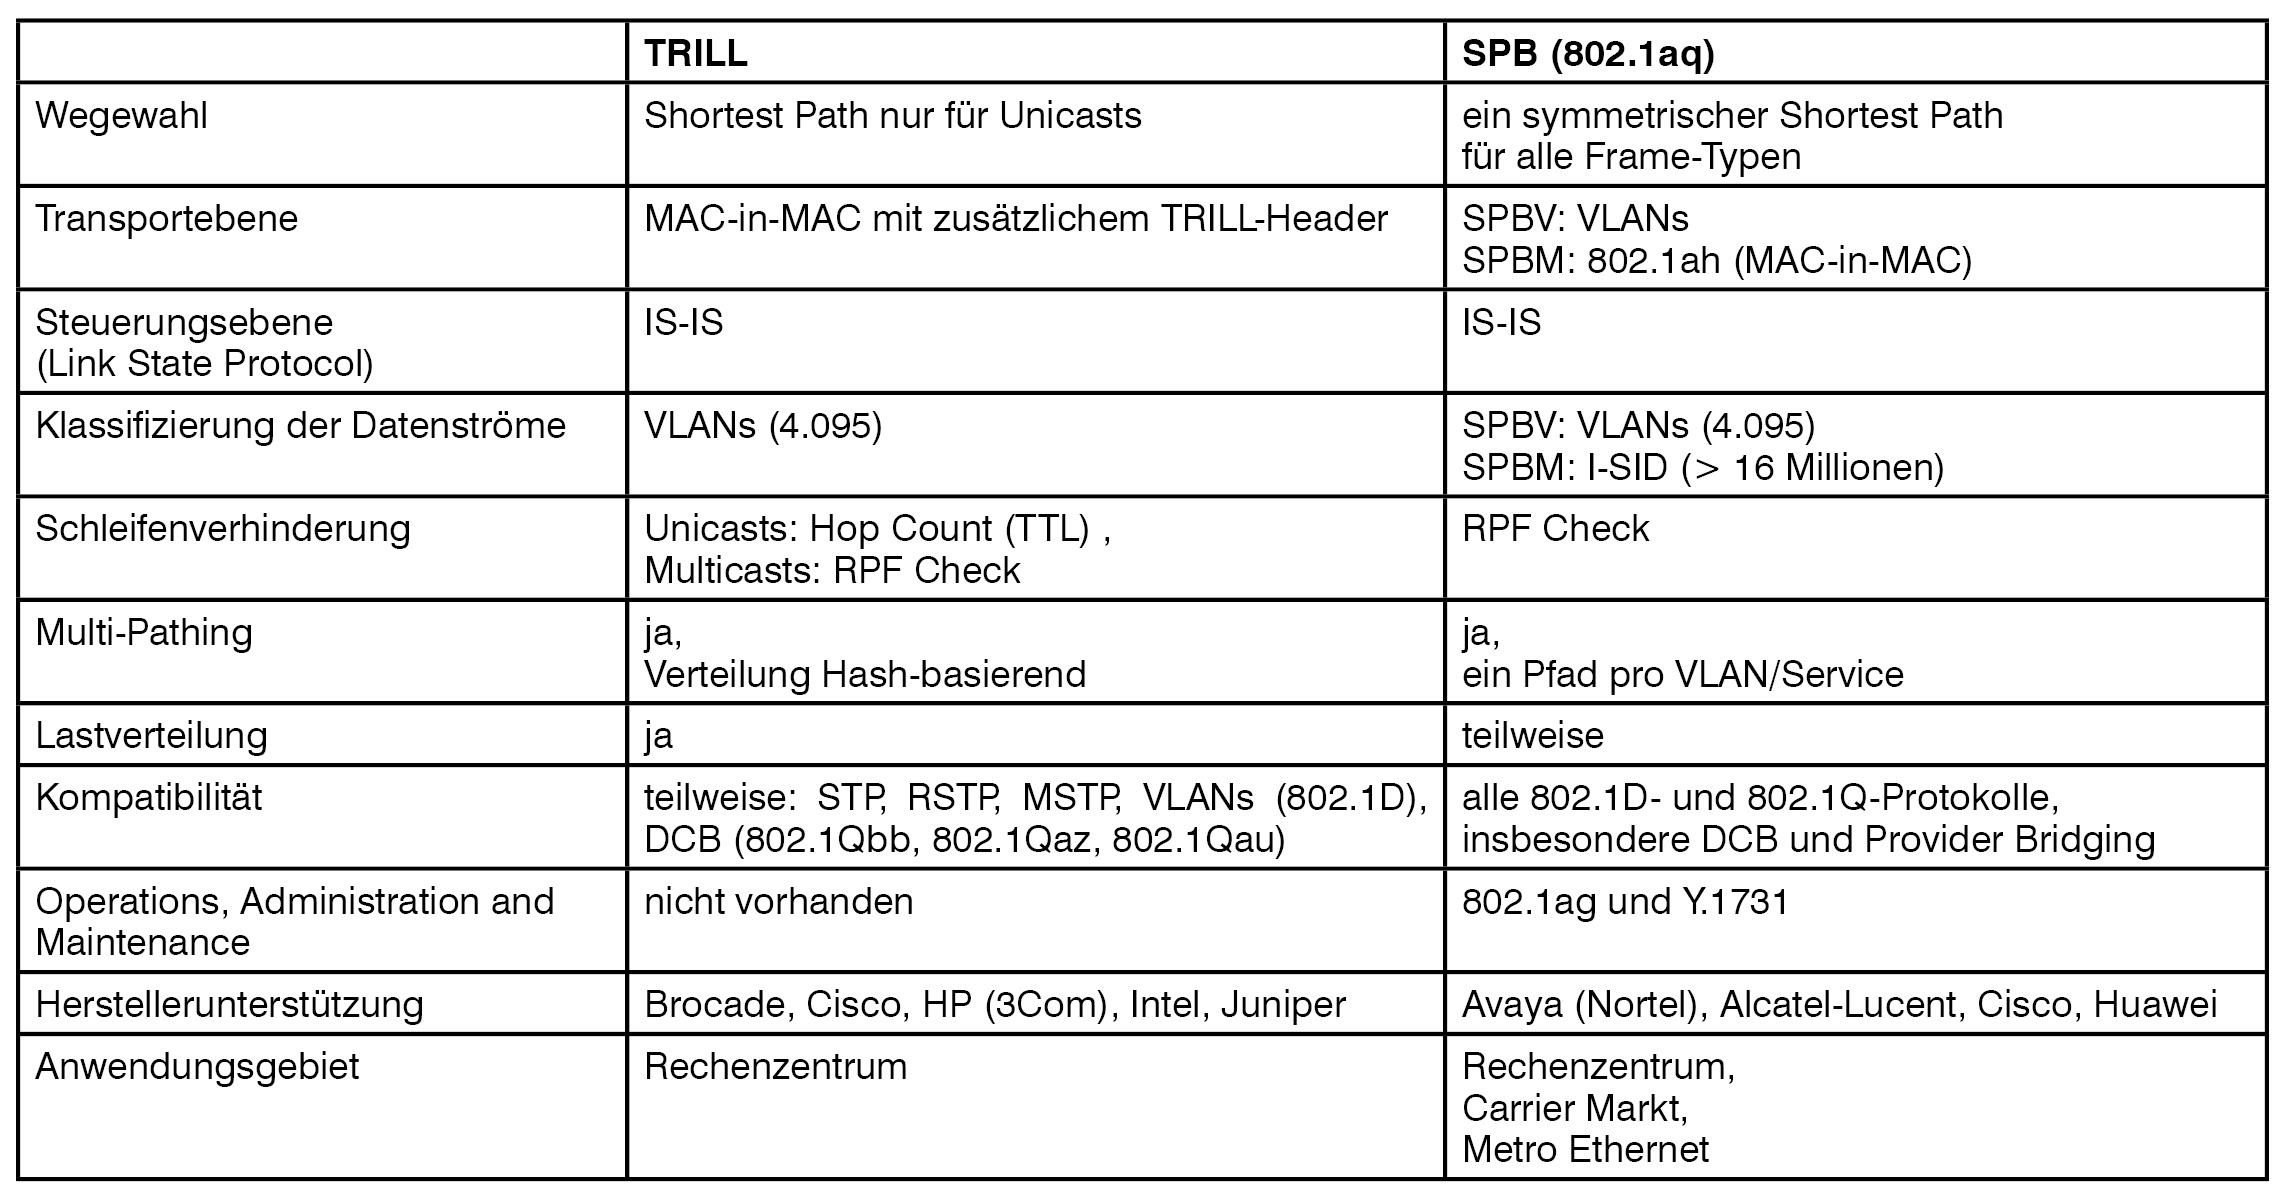
\includegraphics[width=0.80\textwidth]{./pictures/vergleich_spb-trill.jpg}
	\caption{Vergleichstabelle SPB vs. TRILL - Quelle: http://www.comconsult-research.de/shortest-path-bridging/}
	\label{x}
	\end{center}
\end{figure}
\newpage

\subsection{TRILL im LAB}
Wurde aus der Aufgabenstellung entnommen: \\
\\
\textbf{How is TRILL configured in the lab?}
\begin{itemize}
\item Trees
\item PacketFlow
\item MAC learning
\end{itemize}

\noindent \textbf{TRILL with HP Switches}\\
Use this lab to get further information about TRILL by generating traffic, sniffing packets and analyzing the TRILL headers. The lab infrastructure for TRILL uses 4 HP Switches. The Switches are correctly preconfigured. You must not change the configuration!\\ 
\\
To test the setup and to perform measurements you can use the lab computers by connecting them to the HP Switches. Each group should connect 2 computers to the two different leaf switches. Refer to the physical and logical topology below to see which ports you should use.\\
\\
\textbf{Use SSH to connect to the Switch CLI:}\\
\\
\textbf{User: student Password: student}\\
\\
HP1 IP: 10.5.0.11\\
HP2 IP: 10.5.0.12\\
HP3 IP: 10.5.0.13\\
HP4 IP: 10.5.0.14\\
\\
\textbf{Useful CLI Commands:}\\
system-view\\
display trill ?\\
display lldp neighbor-information list\\
display mac-address\\
display ip routing-table\\
\newpage
\textbf{Laboraufbau TRILL: Aufgabenstellung}
\begin{figure} [H]
	\begin{center}
	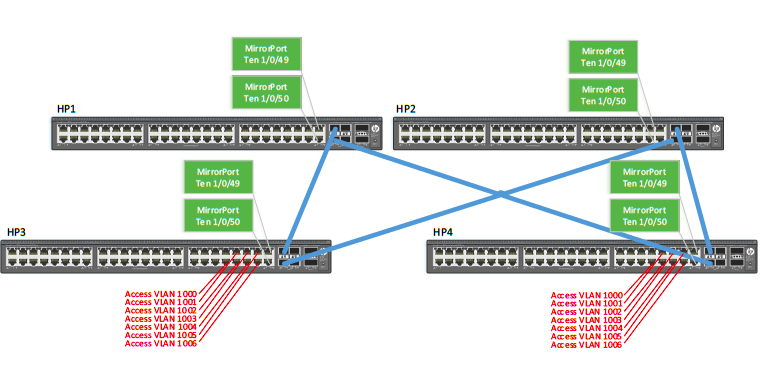
\includegraphics[width=0.80\textwidth]{./pictures/trill_laboraufbau.png}
	\caption{Aufgabenstellung: Laboraufbau TRILL}
	\label{x}
	\end{center}
\end{figure}

\subsubsection{Konfiguration Computer}
Für dieses Lab wurden zwei Computer benötigt. Folgende Konfigurationen waren notwendig: 
\begin{center}
    \begin{tabular}{@{} l l r@{}}\toprule    
    {Computer} & {IP-Adresse} & {Subnetzmaske}\\ \midrule
    PC1 & 10.10.1.11 & 255.255.255.0\\ \addlinespace
    PC2 & 10.10.1.12 & 255.255.255.0\\ 
    \bottomrule
    \end{tabular}
\end{center}

\noindent PC1 wurde an den Switch HP4 angeschlossen, und PC2 an den Switch HP3. 

\subsubsection{Switches}
Für den Laboraufbau wurden vier Switches benötigt. Wurde durch Analyse mit SSH von den Geräten entnommen. Hier einige wichtige Switch-Konfigurationen: 
\begin{center}
    \begin{tabular}{@{} l l r@{}}\toprule    
    {Switch (TRILL-Name)} & {IP-Adresse} & {MAC-Adresse}\\ \midrule
    HP1 (0x2b67) & 10.5.0.11 & 44:21:92:60:62:47\\ \addlinespace
    HP2 (0x56ce) & 10.5.0.12 & 44:31:92:5F:ED:B7\\ \addlinespace
    HP3 (0x8235) & 10.5.0.13 & 44:31:92:60:6D:B8\\ \addlinespace
    HP4 (0xad9c) & 10.5.0.14 & 44:31:92:60:54:78\\
    \bottomrule
    \end{tabular}
\end{center}

\subsubsection{VLAN}
Unsere Computer wurden im VLAN 1006 angeschlossen. 

\subsubsection{Laboraufbau: Gruppe}
Hier folgt das Bild von Samu. 

\subsubsection{TRILL: Diverse Befehle}
Hier folgen Informationen über TRILL mit Hilfe des Kommandos \textit{trill brief}:
\begin{figure} [H]
	\begin{center}
	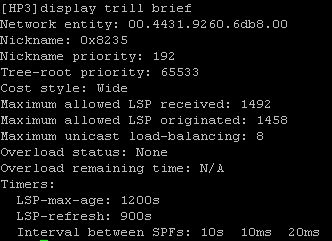
\includegraphics[width=0.80\textwidth]{./pictures/brief.jpg}
	\caption{Screenshot HP3: trill brief}
	\label{x}
	\end{center}
\end{figure}

Mit dem Befehl \textit{trill neighbor table} findet man die Nachbaren heraus: 
\begin{figure} [H]
	\begin{center}
	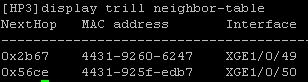
\includegraphics[width=0.80\textwidth]{./pictures/neighbor-table.jpg}
	\caption{Screenshot HP3: trill neighbor-table}
	\label{x}
	\end{center}
\end{figure}
\newpage

\subsubsection{Trees}
Hier einen Überblick über alle Geräte und ihre Nachbaren. Diese Informationen kann man mithilfe von \textit{trill neighbor-table} rauslesen: 
\begin{center}
    \begin{tabular}{@{} l l r@{}}\toprule    
    {Switch} & {Nachbaren}\\ \midrule
    HP1 & HP3 und HP4\\ \addlinespace
    HP2 & HP3 und HP4\\ \addlinespace
    HP3 & HP1 und HP2\\ \addlinespace
    HP4 & HP1 und HP2\\ 
    \bottomrule
    \end{tabular}
\end{center}
Wie ein solcher Eintrag aussieht kann aus der Abbilung 7 entnommen werden. 

\subsubsection{PacketFlow}
Mit Wireshark wurde der packet flow der Switches analysiert. Dadurch konnte festgstellt werden das sporadisch IS-IS Packete durch das Netzwerk fliessen, an eine Multicast Adresse. 
\begin{figure} [H]
	\begin{center}
	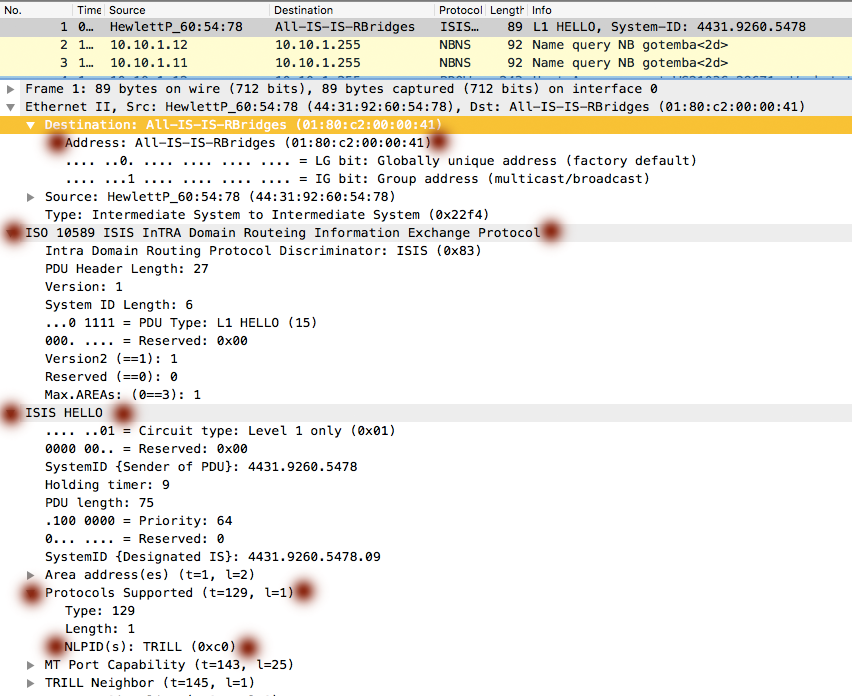
\includegraphics[width=0.80\textwidth]{./pictures/capture_isis.png}
	\caption{Screenshot: Sniff zwischen HP Switches}
	\label{x}
	\end{center}
\end{figure}
\noindent Aus diesem Screenshot kann man erkennen das es sich um ein IS-IS HELLO Packet handelt, dass an die Multicast Adresse \textit{All-IS-IS-RBridges} gesendet wird. Weiter unten ist auch zu erkennen, dass es sich um TRILL handelt (supported protocols). 
\newpage
Bei einem weiteren Sniff Versuch, wurde von PC1 zu PC2 gepingt. 
\begin{figure} [H]
	\begin{center}
	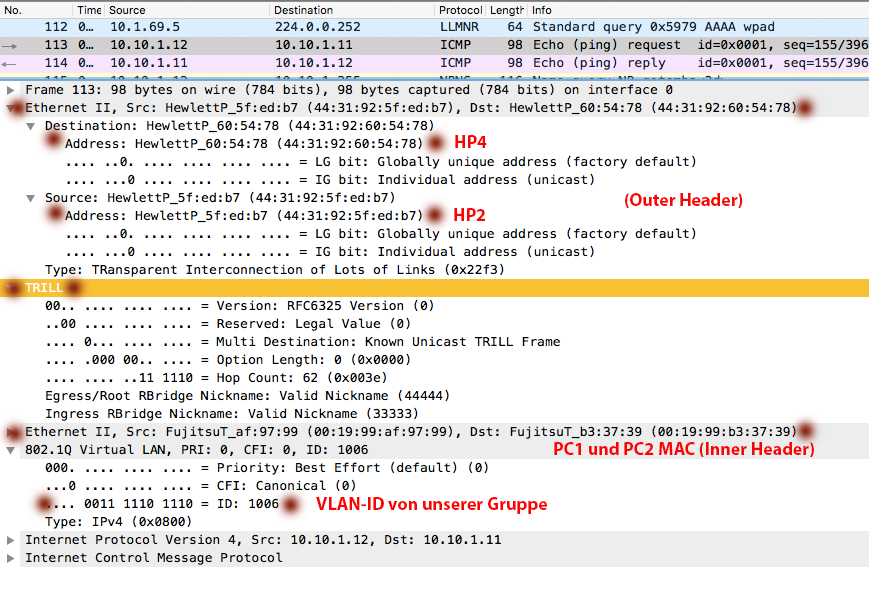
\includegraphics[width=0.80\textwidth]{./pictures/capture_ping.png}
	\caption{Screenshot: Sniff zwischen HP Switches (Ping Request)}
	\label{x}
	\end{center}
\end{figure}
\noindent Bei dieser Abbildung handelt es sich um einen Wireshark Ausschnitt, während PC2 den PC1 anpingt. Hier ist schön zu erkennen dass das Ethernet Frame eingepackt wird. Der Inner Ethernet Header wird nicht verrändert und enthält die MAC-Adressen der beiden PCs. Im Outer Ethernet Header sieht man die Informationen der HP Switches die das Frame empfangen und weiterleiten. Der zu empfangende Switch entfernt den TRILL Header und somit den Outer Ethernet Header und leitet das Packet an den PC weiter. \\\\
Ein weiterer Test zeigte sich das die Frames nicht immer über den HP2 Switch fliessen müssen, sondern können ebenso über den HP1 fliessen.  Um dies zu testen haben wir auf \textit{ping} verzichtet und haben ein anderes Tool genommen das über TCP kommuniziert: \textit{jperf}. Damit wird ein neuer Hash  berechnet, da andere Protokolle im Einsatz sind, und die wahrscheinlichkeit ist sehr hoch das die Packete eine andere Route folgen (Da die Route meistens anhand von einem Hash über alle Informationen gewählt wird). Leider existieren von diesem Test keine Screenshots, die es beweisen würden. Es wurde jedoch ausführlich getestet.  

\subsubsection{MAC Learning} 
Das MAC-learnig bei RBridges ist sehr ähnlich wie bei normalen Switches, mit einigen Differenzen. Eine Ingress RBrigde welche ein Packet von einem Client erhält, notiert die MAC-Adresse des Clients (welche im Inner Ethernet Header steht) in seine MAC-Tabelle. Nach diesem Vorgang müsste die Ingress RBridge das Packet an eine Engress RBridge weiterleiten, es kann jedoch sein das die Engress RBridge welche das Packet erhalten soll (Inner Ethernet Header Destination Adresse des Clients) noch nicht bekannt ist. So flooded die Ingress RBridges anhand von Multicast Frames (ALL-RB-MCAST) einen Request aus an alle RBridges im Netz. Die RBridge die auf den Request antwortet kennt die MAC-Adresse der Destination MAC-Adresse des Clients (Inner Ethernet Header) und meldet sich bei der Ingress RBridge. Die Engress RBridge notiert die MAC-Adressen in seine table und kennt somit die Ingress RBridge jetzt. 

\newpage
\section{VXLAN - Teil 2}
VXLAN steht für Virtual eXtensible Local Area Network und ist einer der IETF festgelegten Standard. 
\subsection{Funktion}
Es handelt sich um ein Encapsulation-Protokoll, dass es erlaubt ein Overlay Netzwerk auf einer existierender Layer 3 Umgebung laufen zu lassen. VXLAN erzeugt logische Layer 2 Netzwerke die dann in Layer 3 Packete eingepackt werden. Dank VXLAN kann man ein Netzwerk extrem skalieren. Dies ist vorallem in einem Rechenzentrum, oder Rechenzentrum übergreifend, notwendig, wo viele Tenants sich ein pyhsiches Netzwerk teilen. Ein Problem vor der Einführung von VXLAN war, dass die Netze via VLANs getrennt wurden. Da es maximal 4096 VLANs per Netz geben konnte, war man sehr eingeschränkt und in grossen Umgebungen war das nicht genug. VXLAN wurde primär entwickelt um dieses Problem zu lösen (Erweiterung von VLANs). Für diesen Zweck hat man ein Segment mit 24 Bit hinzugefügt. Dies bedeutet das dank VXLAN nicht nur 4096 Netzwerk IDs verteilt werden können, sondern über 16 Millionen. 

\subsubsection{VNI}
Dank der VXLAN Encapsulation wird jedes ausgehende Frame mit VXLAN Header eingepackt der das VXLAN mit einer VNI identifiziert. Diese ist vergleichbar mit dem bekannten VLAN-Tag. 

\subsubsection{VTEP}
Wenn man von VTEP redet, dann meint man damit die VXLAN fähige Endgeräte. Diese können physisch sowie virtuell sein. Eine VM die sich hinter einem VTEP befindet, wird dynamisch von dem jeweiligem VTEP gerlernt. 

\subsubsection{MTU}
Ein Problem das auftauchen könnte ist die MTU im jeweiligen Netzwerk, zwischen den VTEPs. VXLAN Packete dürfen nicht fragmentiert werden, da diese ansonsten von der zu empfangenden VTEP verworfen werden. Es ist wichtig zu achten das genügend MTU berechnet wird. 

\subsubsection{Data Flow}
Verbindung zwischen zwei VMs im gleichem VXLAN: 
\begin{enumerate}
\item VM1 will mit VM2 kommunizieren 
\item VM1 sendet ein ARP Request 
\item VTEP1(VM1 befindet sich dahinter) nimmt Request entgegen 
\item VTEP1 entpackt den Request mit VXLAN Header 
\item VTEP1 versendet Request per Multicast 
\item VTEP2 nimmt Request entgegen, da VM2 dahinter ist 
\item VTEP2 lernt dass VM1 sich hinter VTEP1 befindet 
\item VTEP2 entpackt Frame und sendet Packet weiter zu VM2
\item VM2 erhält ARP Layer 2 Packet, merkt nichts von VXLAN
\end{enumerate}

\subsubsection{Learning Table}
Die VTEP behalten Einträge solange wie die TTL gültig ist. Danach wird dieser entfernt. Das learning erfolgt dynamisch. EIne solche Tabelle beinhaltet die VM MAC, dazugehöriges VXLAN und den VTEP. 

\subsubsection{Gateway}
Um zwischen VXLAN kommunizieren zu können, ist ein VXLAN-Gateway erfolderlich. Dieser ist ebenfalls fähig VXLAN Header zu entfernen oder hinzuzufügen. Durch dies können Packete auch in ein nicht VXLAN-fähiges Netzwerk gesendet werden. 

\subsection{Header}
Folgende Abblidung zeigt ein VXLAN-Packet. 
\begin{figure} [H]
	\begin{center}
	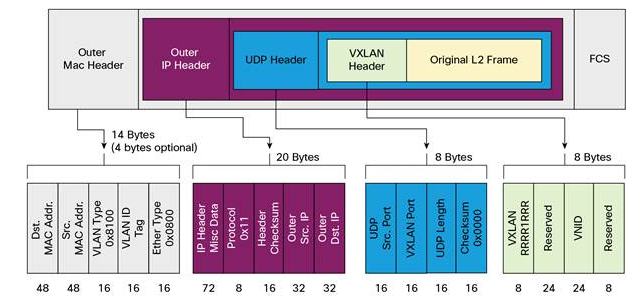
\includegraphics[width=0.80\textwidth]{./pictures/vxlan_header.png}
	\caption{Cisco Abbildung eines VXLAN-Frames}
	\label{x}
	\end{center}
\end{figure}
\noindent Aus dieser Abbildung ist zu erkennen dass auf L2 Frame ein VXLAN Header hinzugefügt bekommt, und das ganze in ein UDP Packet gepackt wird. Dies führt zu erhöhtem Overhead. Deswegen ist die Wahl der MTU Size sehr wichtig. 

\subsubsection{Felder}
Sehen wir uns den VXLAN Header genauer an: 
\begin{figure} [H]
	\begin{center}
	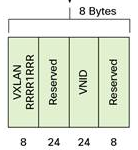
\includegraphics[width=0.30\textwidth]{./pictures/vxlan_header_detail.png}
	\caption{Cisco Abbildung - Detail Ansicht VXLAN Header}
	\label{x}
	\end{center}
\end{figure}

Der VXLAN Header beinhaltet 8 Bytes und ist folgendermassen aufgebaut: 
\begin{itemize}
\item Flags: 8 Bit 
\item Reserved: 24 Bit 
\item VNI ID: 24 Bit 
\item Reserved: 8 Bit 
\end{itemize}

\subsection{Ziele von VXLAN?}
Das primäre Ziel von VXLAN ist es die Kapazität von VLAN zu erweitern. Es wurde entwickelt um die Skalierbarkeit in einem Rechenzentrum zu gewährleisten. Mit VXLAN kann eine multitenancy-Fähigkeit in einem Rechenzentrum oder Rechenzentrum übergreifend gewährleistet werden, somit können VMs sich im gleichem Layer 2 Netzwerk befinden. 

\subsection{Warum wurde VXLAN entwickelt?}
VXLAN wurde primär entwickelt um VLAN zu erweitern. Mehr zum Einsatz findet man im Kapitel Ziele von VXLAN. 

\subsection{Wo und Wie kann VXLAN verwendet werden?}
Hier einige Anwendungsbeispiele von VXLAN: 
\begin{itemize}
\item VM Verschieben: Nehmen wir an wir möchten gerne eine neue VM auf einem physischen Server implementieren, die Kapazität von diesem reicht jedoch nicht aus. Es können VMs auf andere Server gezügelt werden und diese verbleiben im gleichen Layer 2 Netzwerk. 
\item Rechenzentrum Kapazität: DIe Kapazität von VLANs ist auf 4096 begrenzt. Für manche Rechenzentren reicht diese nicht aus. Da kommt VXLAN ins Spiel. Dank VXLAN ist die Grenze von 4096 Netzwerk IDs aufgehoben, und es können neu bis zu 16 Millionen Netzwerk IDs vergeben werden. 
\item Ein Kunde möchte seine Umgebung auf mehrere Rechenzentren spalten, es besteht jedoch das Problem das sich die VMs nicht im gleichen Layer 2 Netzwerk befinden würden. Dank VXLAN ist eine solche Implementation möglich. Es ermöglicht dem Kunden eine Rechenzentrum übergreifende Layer 2 Umgebung. 
\end{itemize}

\subsection{Vergleich von VXLAN mit traditionelle Protokolle}

\subsection{Welche Vor- und Nachteile bringt VXLAN mit sich?}

\subsubsection{Vorteile}

\subsubsection{Nachteile}

\subsection{Ähnliche Technologien wie VXLAN?}

\subsubsection{coming soon}

\subsection{VXLAN im LAB}

\end{document}
